\documentclass[11pt,a4paper]{article}
\usepackage[paper=a4paper,left=25mm,right=20mm,top=30mm,bottom=30mm]{geometry} 
\usepackage[english, ngerman]{babel}
\usepackage[utf8]{inputenc}
\usepackage[colorlinks=false]{hyperref}
\usepackage[table,usenames,dvipsnames]{xcolor}
\usepackage{tabularx}
\usepackage{graphicx}
\usepackage{subfigure}
\usepackage{listings}
\usepackage{float}
\usepackage{hyperref}
\usepackage{multicol}
\usepackage{fancyhdr}
\usepackage{sectsty}
\usepackage[final]{pdfpages}
\usepackage{threeparttable}
\usepackage{amsmath}
\usepackage{tikz}
%\usepackage{gitinfo}
\usepackage{totpages}
\usepackage{datetime}
\usepackage[printonlyused]{acronym}
%\usepackage{syntonly}
%\syntaxonly
  
%Definitionen
\includepdfset{pages=-} %Alle Seite importieren  Option: noautoscale
\setlength{\parindent}{0em} %Einrueckung eines neuen Absatzes, 0 keine Einrueckung

\definecolor{rowc1}{RGB}{40,75,95}

\setcounter{tocdepth}{3}
\setcounter{secnumdepth}{3}

\ifpdf
\pdfinfo {
	/Author (Marc Schärer, Arthur van Ommen, Fabian Affolter)
	/Title (Report)
	/Subject ()
	/Keywords ()
	/CreationDate (D:\pdfdate)
}
\fi

\pagestyle{fancy}
\renewcommand{\headrulewidth}{0pt}
\lhead{}%\includegraphics[width=80mm]{logo.png}}
\chead{}
\rhead{}
\lfoot{}
\cfoot{\thepage}
\rfoot{}

\definecolor{mygreen}{rgb}{0,0.6,0}
\definecolor{mygray}{rgb}{0.5,0.5,0.5}
\definecolor{mymauve}{rgb}{0.58,0,0.82}

\lstset{ %
  backgroundcolor=\color{white},   % choose the background color; you must add \usepackage{color} or \usepackage{xcolor}
  basicstyle=\footnotesize,        % the size of the fonts that are used for the code
  breakatwhitespace=false,         % sets if automatic breaks should only happen at whitespace
  breaklines=true,                 % sets automatic line breaking
  captionpos=b,                    % sets the caption-position to bottom
  commentstyle=\color{mygreen},    % comment style
  deletekeywords={...},            % if you want to delete keywords from the given language
  escapeinside={\%*}{*)},          % if you want to add LaTeX within your code
  extendedchars=true,              % lets you use non-ASCII characters; for 8-bits encodings only, does not work with UTF-8
  frame=single,                    % adds a frame around the code
  keepspaces=true,                 % keeps spaces in text, useful for keeping indentation of code (possibly needs columns=flexible)
  keywordstyle=\color{blue},       % keyword style
  language=Octave,                 % the language of the code
  morekeywords={*,...},            % if you want to add more keywords to the set
  numbers=left,                    % where to put the line-numbers; possible values are (none, left, right)
  numbersep=5pt,                   % how far the line-numbers are from the code
  numberstyle=\tiny\color{mygray}, % the style that is used for the line-numbers
  rulecolor=\color{black},         % if not set, the frame-color may be changed on line-breaks within not-black text (e.g. comments (green here))
  showspaces=false,                % show spaces everywhere adding particular underscores; it overrides 'showstringspaces'
  showstringspaces=false,          % underline spaces within strings only
  showtabs=false,                  % show tabs within strings adding particular underscores
  stepnumber=2,                    % the step between two line-numbers. If it's 1, each line will be numbered
  stringstyle=\color{mymauve},     % string literal style
  tabsize=2,                       % sets default tabsize to 2 spaces
  title=\lstname                   % show the filename of files included with \lstinputlisting; also try caption instead of title
}

\renewcommand{\arraystretch}{1.3}

\lstset{basicstyle=\ttfamily,breaklines=true}

\begin{document}
%PRE DOCUMENT STUFF%%%%%%%%%%%%%%%%%%%%%%%%%%%%%%%
\input{title}

\pagenumbering{Roman} % Seitennummerierung durch roemische Ziffern
\include{toc}
%%\begin{abstract}
\section*{Zusammenfassung}
%
Das Hochregallager ist ein Lagerungssystem, welche sich mit einer hohen Lagerdichte und Wirtschaftlichkeit von anderen Konzepten abhebt...\newline


%
% %EOF

\pagenumbering{arabic} % Seitennummerierung durch arabische Ziffern
\clearpage

%%%%%%%%%%%%%%%%%%%%%%%%%%%%%%%%%%%%%%%%%%%%%%%%%
\section{Einleitung}
Ein Hochregallager (HRL) beschreibt ein Lagersystem mit Plätzen in sogenannten Regalen. Hochregallager gibt ein in den unterschiedlichsten Ausprägungen. Die grössten Ausführungen besitzen Höhen bis etwa 50 m und können mehreren hunderttausend Plätze besitzen. Oftmals werden direkt Euro-Paletten als Träger für das Lagergut verwendet, ist das Lagergut zu klein, werden häufig spezielle Kunststoff-Behälter benutzt.\\
Grobgesagt besteht ein Hochregallager aus einer bestimmten Anzahl von Gassen. Eine Gasse wiederum hat links und rechts Lagerplätze und im Freiraum bewegt sich ein Bediengerät. In einem manuellen Hochregallager ist dieser Raum so gross, dass mit einem Gabelstapler zwischen den Regalwänden manövriert werden kann. Bei automatischen Lagern fährt ein Bediengerät, welches von einem Lagerverwaltungssystem seine Befehle bekommt, ohne manuelle Interventionen in der Gasse und liefert das Lagergut zur Entnahmestelle.\\
Die Hochregallager haben eine hohe Raumnutzung und bei der Erstellung sind hohe Investitionen nötig, da bei kleiner Ausführungen eine Halle um das Hochregallager gebaut werden muss. Bei grossen Varianten wird das Hochregal als Tragstruktur für das Gebäude mitbenutzt. 

%
\subsection{Rahmenbedingungen}

%
\subsection{Abgrenzung}
Die Schnittstelle liegt an der Stirnseite des Hochregallagers zur Vorzone.


%EOF

\section{Grundlagen}
Im Sinne eines Hochregallager besteht eine Gasse aus einer rechten und einer linken Regalwand während sich in der Mitte der beiden Wände ein Korridor für das Regalbediengerät befindet. Die Regalwände sind in Lagerplätze unterteilt, die von Regalbediengerät be- und entladen werden. Hochregallager können aus einer beliebigen Anzahl Gassen bestehen. Im Normalfall befindet sich an einer Stirnseite der Gassen die sogenannte Vorzone, welche die Aufgabe hat, die Lagergüter auf die zugeweisen Gassen zu verteilen. 
%
\begin{figure}[h]
  \begin{center}
    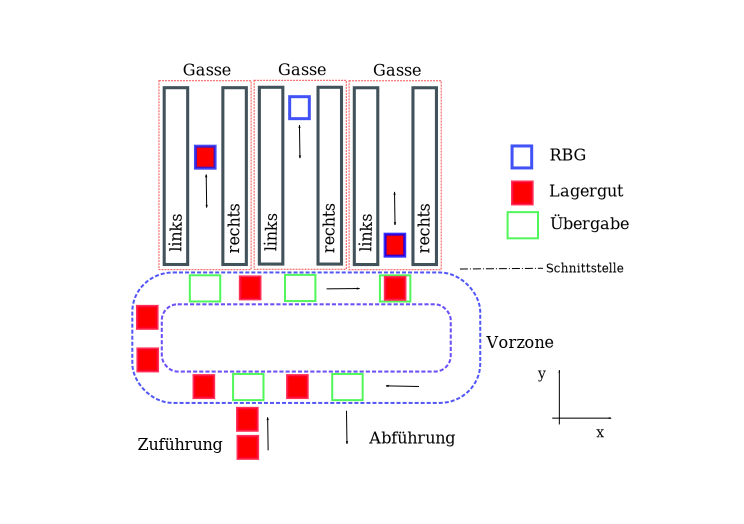
\includegraphics[width=0.9\textwidth]{images/uebersicht.png}
    \caption{Übersicht}
    \label{fig:overview}
  \end{center}
\end{figure}
%

%
\subsection{Allgemeine Grundlagen}



%

\subsubsection{Koordinaten}
Der Koordinatenursprung befinet sich in der linken unteren Ecke der Regalwand. Es wird yz-Koordinatensystem aufgespannt und die Koordinaten der Lagerplätze (Bins) in die linke untere Ecke gesetzt. Das Regalbediengerät kann sich auf der y- und der z-Achse bewegen. Der Übergabebereich befindet sich ausserhalb des Koordinatensystems auf den negativen Abschnitt der y-Achse. 
%
\begin{figure}[h]
  \begin{center}
    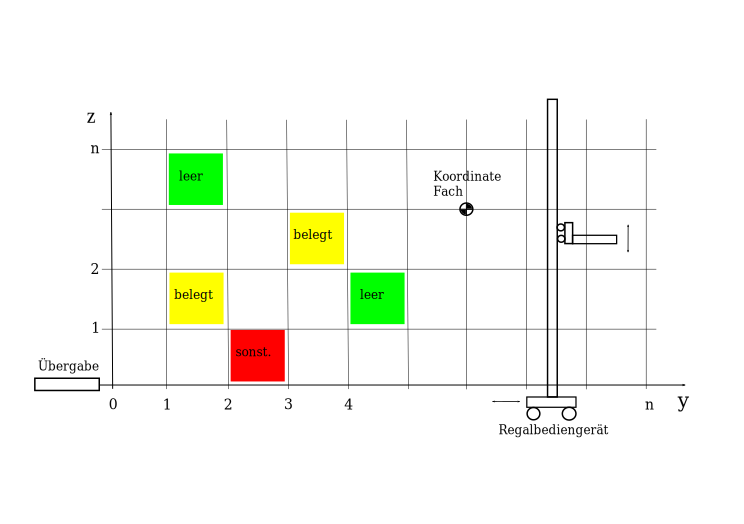
\includegraphics[width=0.9\textwidth]{images/koordinaten-wand.png}
    \caption{Lagerwand}
    \label{fig:wand}
  \end{center}
\end{figure}
%
In Abbildung \ref{fig:wand} sind ebenfalls die verwendete Farbzuordung für die Lagerplätze (Bins) ersichtlich.
%
\begin{table}
  \caption{Farbzuordung Lagerplätze}
  \label{tab:bin-color}

  \begin{center}
    \begin{tabular}{cc}
       grün & leer\\
       gelb & belegt\\
       rot & reserviert/defekt/spezial \\
    \end{tabular}
  \end{center}
\end{table}

%
\subsubsection{Klappung}
Für die zweidimensionale Darstellung wurde eine Lagergasse gemäss Abbildung \ref{fig:klapp} aufgefaltet, respektive aufgeklappt.
%
\begin{figure}[h]
  \begin{center}
    
\includegraphics[width=0.9\textwidth]{images/klappung.png}
    \caption{Klappung}
    \label{fig:klapp}
  \end{center}
\end{figure}

%
\subsection{Mathematische Grundlagen}
Regalbediengerät bewegt sich zwischen den Lagerwänden auf der y- und der z-Achse. Der Arm des Regalbediengerät verfährt auf der y-Achse und der Ausleger auf der z-Achse. Die Bewegungen auf beiden Achsen lassen somit beliebige Verfahrwege auf der yz-Ebene zu. 
%
\begin{equation}
\alpha = \arcsin \frac{f}{\sqrt{a-v} * \vec{b} + d_{g}}
\end{equation}



%
\subsection{Simulationstechnische Grundlagen}





%EOF


\section{Modellierung}
Der Aufbau des Hochregallagers wurde in diverse Bereiche unterteilt. Die wichtigsten sind das Hochregal selbst, wie auch das Regalbediengerät. Weitere sind die entsprechenden Zustände/Ereignisse, die innerhalb des Hochregallagers auftreten können. 
%
\subsection{Einheiten}
Die Basiseinheit ist Milimeter. Es ist jedoch möglich mit anderen SI-Einheiten (m, dm oder cm) zu arbeiten.
%
\subsection{Hochregal}
Das gesamte Hochregallager, oder auch der Lagerort, wird durch ein einzelnes Objekt dargestellt. Dieses Objekt enthält alle benötigten Informationen und ist als Singleton implementiert. Das heisst, dass auf die Gassen, das Regal und die Lagerfächer direkt zugegriffen werden kann. Dies bietet eine komfortables Arbeiten bei der Simulation und soll auch eine einfache Implementierung der Visualisierung ermöglichen. Weiter bietet es den Vorteil, dass alle Informationen über die Elemente des Lagerortes immer verfügbar sind und abgefragt werden können. Mit GetInstance() und den entsprechenden Get-Methoden des jeweils untergeordeneten Objekts kann auf jedes einzelne Element des Lagerorts zugegriffen werden.
%
\subsection{Regalbediengerät}
Innerhalb der Gasse bewegt sich nur das Regalbediengerät. Die Klasse RackFeeder bildet dies ab. Im vorherigen Abschnitt wurde auf die zulässigen Bewegungen eingegangen. Die maximalen Beschleuigungen, Verzögerungen und die Geschwindigkeit sind innerhalb dieser Klasse als Standardwerte definiert. Bei Bedarf lassen sie sich überschreiben.\\
Das Regalbediengerät (RackFeeder) kann nicht beliebige Bewegungen auchführen. Die einzig gültigen Bewegungen sind durch ein vollständiges Objekt definiert, es sind nur drei Bewegungen zulässig: 
%
\begin{itemize}
  \item Bewegung in yz-Achse
  \item Bewegung in x-Achse (dies ist vorhanden, jedoch wird es nicht verwendet, da in der Realität die Operationen in der Vorzone von einem zusätzlichen System wahrgenommen werden)
  \item Bewegung in u-Achse (in das Regalfach hinein zum Be- und Entladen des Lagergütes)
\end{itemize}
%
Dies verhindert, dass der RackFeeder physikalisch unmögliche Bewegungen ausführen kann und stellt sicher, dass in jedem Zustand nur die darin gültigen Bewegungen ausgeführt werden können.
%
\subsection{Ereignisse}
Innerhalb des Systems wurden die Ereignisse (Events) in die Operationen Einlagern und Auslagern zerlegt. Die Verzweigungen sind in den nachfolgenden Abbildungen in gelb dargestellt. Der Startpunkt ist blau und entspricht dem Verhalten im Wartemodus. 
%
\begin{figure}[H]
\subfigure[Einlagern]{\includegraphics[width=0.49\textwidth]{images/einlagern.png}}\hfill
\subfigure[Auslagern]{\includegraphics[width=0.49\textwidth]{images/auslagern.png}}
\caption{Verhalten}
\end{figure}
%
Die nachfolgende Tabelle zeigt auf der linken Seite die Einlagerung und auf der rechten Seite die Auslagerung.
%
\begin{table}[H]
  \caption{Events}
  \label{tab:event}
  \begin{center}   
    \begin{tabular}{ccc|c|ccc}
		Eventnr.&	Koord.&	Zustand & & Eventnr.&	Koord.&	Zustand\\
		\hline
		1 &			0/0 &	empty & & 1 &			0/0 	&empty\\
		2 &			0/0 &	loaded & & 6 &			y/z 	&empty\\
		3 &			y/z &	loaded & & 5 &			x 		&empty\\
		4 &			x 	&	loaded & & 4 &			x 		&loaded\\
		5 	&		x 	&	empty & & 3 &			y/z 	&loaded\\
		6 	&		y/z &	empty & & 2 &			0/0 	&loaded\\
		1	&		0/0	&	empty & & 1	&		0/0		&empty\\
		7 &					&sleep& & 7 &					&sleep\\
    \end{tabular}
  \end{center}
\end{table}
%	
\subsection{Architektur}
Die Unterteilung der Anwendung erfolgte in einen Teil für die Modellierung, einen für die Simulation und einen für die Visualisierung. Diese Trennung macht die Anwendung in Bezug auf geänderte Lagerorte und Simulationensszenarien, oder auch für Optimierungen flexibel.
%
%
\begin{figure}[H]
  \begin{center}
    \includegraphics[width=0.8\textwidth]{images/package_diagramm.png}
    \caption{Package-Diagramm}
    \label{fig:packages}
  \end{center}
\end{figure}
%
\begin{figure}[H]
  \begin{center}
    \includegraphics[width=0.8\textwidth]{images/class_diagramm.png}
    \caption{Class-Diagramm}
    \label{fig:class}
  \end{center}
\end{figure}
%
Die weiteren Diagramme befinden sich im Anhang.


%EOF

\section{Simulation}
\subsection{Allgemein}
Die Simulation wurde als ereignisgesteuerte Echtzeitsimulation implementiert. Die Basis sind Lageraufträge wie Einlagerungs-, Auslagerungs- und Umlagerungsaufträge. Zu Beginn der Simulation muss (momentan) mindestens 1 Auftrag vorhanden sein, da die leere Auftragsliste, bzw. die daraus resultierende leere Ereignisliste, das Abbruchkriterium ist, um die Simulation zu beenden. Dies könnte noch verbessert werden, indem die gewünschte Simulationsendzeit als Erinnerungsereignis in die Ereignisliste eingetragen würde. Die Simulation würde dann nach Abarbeitung dieses letzten Erinnerungsereignisses gestoppt, sofern mittlerweile keine noch späteren Ereignisse eingetragen wurden. \\
Es könnten während der laufenden Simulation weitere Aufträge hinzugefügt werden. Die Startzeit des Auftrags muss allerdings die aktuelle Simulationszeit übersteigen. Bei der Eingabe von zusätzlichen Aufträgen ist das Zeitformat zu berücksichtigen. Diese Funktion ist momentan nicht implementiert.
\\
Für jeden zukünftigen Auftrag wird ein Erinnerungsereignis in die Ereignisliste eingetragen mit Ereigniszeit = Startzeit des Auftrags. Dies dient dazu, dass die Simulation selbst nur die Ereignisliste abarbeiten kann, indem die Simulation jeweils das früheste Ereignis aus der Liste entfernt, anhand der Simulationszeit die benötigte Wartezeit berechnet und dann exakt zur richtigen Simulationszeit das Ereignis ausführt. In der Regel führt jedes Ereignis zu einem Nachfolgeereignis, welches
wiederum in die Ereignisliste eingetragen wird. Dieser Vorgang wird solange wiederholt, bis die Ereignisliste leer ist, wodurch die Simulation beendet wird.
%
\subsection{Spezialfälle}
Einzig das letzte Ereignis eines Auftrags sowie unter Umständen ein Erinnerungsereignis können dazu führen, dass kein Nachfolgeereignis mehr erstellt wird. Dies ist der Fall, wenn für die aktuelle Gasse keine weiteren Aufträge mehr vorhanden sind oder überhaupt keine Aufträge mehr zur Abarbeitung bereitstehen.\\
Würden keine Erinnerungsereignisse generiert, sondern direkt das erste Ereignis des entsprechenden Auftrags, wäre es schwierig  zusätzliche Aufträge, die vor dem anderen Ereignis starten, in die Ereignisliste einzufügen und diese Liste entsprechend zu bereinigen.\\
Dies wäre aber notwendig, da ansonsten zwei unterschiedliche Aufträge in derselben Gasse parallel ausgeführt würden. Dies ist aber physikalisch unmöglich und darf in der Simulation nicht geschehen! Bei jedem Erinnerungsereignis wird deshalb nur die Auftragsliste auf fällige Aufträge geprüft und bei Bedarf das erste Ereignis für diese Aufträge generiert. Es werden aber nur Ereignisse generiert für Aufträge von Gassen, welche nicht bereits durch andere, momentan ausgeführte Aufträge blockiert sind. Für diese Prüfung wird wiederum die Ereignisliste herangezogen.\\
%
\subsection{Berechnung Simulationszeit}
Die aktuelle Simulationszeit wird anhand folgender Formel berechnet:\\
\begin{equation}
   \begin{split}
 Aktuelle Simulationszeit [ms] = Simulationsstartzeit [ms] \\
  + Faktor * (Aktuelle Systemzeit [ms] – Startsystemzeit [ms])
     \end{split}
\end{equation}
\\
Da im Modus \textit{As Fast As Possible} nicht auf die exakte Ausführungszeit gewartet werden soll, sondern die Ereignisse sofort ausgeführt werden sollen, wird die Formel mit einem Korrekturwert ergänzt, welcher der Summe der Wartezeiten entspricht:
\\%
\begin{equation}
   \begin{split}
Aktuelle Simulationszeit [ms] = Simulationsstartzeit [ms] \\
  + Faktor * (Aktuelle Systemzeit [ms] – Startsystemzeit [ms]) + Korrekturwert [ms]
     \end{split}
  \end{equation}
\\%
Der Korrekturwert bleibt bei der Echtzeitsimulation immer 0, weshalb für beide Simualtionsmodi dieselbe Formel verwendet werden kann.
%
\subsection{Fehler durch Rechenzeit und dessen Kompensation}
Es gibt nun aber Fälle, in denen die Ereignisse anhand der aktuellen Simulationszeit zu spät ausgeführt werden. Dies kommt daher, dass mehrere Ereignisse die gleiche oder zumindest eine kurz aufeinanderfolgende Startzeit haben. Der Grund für die Verzögerung ist, dass ja das \textit{ausführen} der Ereignisse Rechenzeit benötigt und die Berechnung der aktuellen Simulationszeit auf der Systemzeit beruht. Diese Verzögerungen würden sich summieren und müssen unbedingt kompensiert werden.\\
Also wird für die Nachfolgeereignisse nicht die aktuelle Simulationszeit als Basis zur Berechnung der Startzeit des Nachfolgeereignisses verwendet, sondern die Startzeit seines Vorgängerereignisses. Die aktuelle Simulationszeit wird also nur verwendet, um die Wartezeit bis zur Ausführung des nächsten Ereignisse zu berechnen und um zu jedem Zeitpunkt der Simulation den entsprechenden Zustand bzw. die aktuellen Koordinaten der Regalbediengeräte zu berechnen
%
\subsection{Mögliche Strategien}
Für die Simulation gibt es unterschiedliche Strategien, welche das Verhalten des Lagers beinflussen. Neben den Teilen für das Hochregallager selber, gäbe es auch Punkte, die nur das Regalbediengerät berücksichtigen.
%
% \begin{itemize}
%  \item Bewegungsstrategien
%  \begin{itemize}
%   \item Einlagerung
%   \item Auslagerung
%   \item kombiniert
% \end{itemize}
%  \item Ruhepositionsstrategien
%  \begin{itemize}
%   \item Verweilen am letzten Arbeitspunkt
%   \item Rückkehr zur Übergabestelle
%   \item Freie Posistion in der Regalgasse
% \end{itemize}
%  \item Einlagerugnsstrategien
%  \begin{itemize}
%   \item zufällige Einlagerung
%   \item Einlagerung nahe der Auslagerung
%   \item chaotische Einlagerung
%   \item zonierte Einlagerung
% \end{itemize}
%  \item Auslagerugnsstrategien
%  \begin{itemize}
%   \item strenges FIFO
%   \item abgeschwächtes FIFO
% \end{itemize}
%  \item Umlagerungsstrategien
%  \begin{itemize}
%   \item keine Umlagerungen
%   \item zufällige Umlagerungen
%   \item zonierte Umlagerung
% \end{itemize}
%  \item Reihenfolgestrategien
%  \begin{itemize}
%   \item First come, first serve
%   \item Fahrweg- und Zeit-Optimierung
%   \item lokale Queue-Optimierung
%   \item globale Optimierung
% \end{itemize}
%  \item Nichtbeschäftigungsstrategien
% \end{itemize}
%
Im momentan Stand wird das Regalbediengerät, als Ruhepositionsstrategien, immer wieder auf die Warteposition bei der Vorzone gesetzt. Ohne statistische Daten einer Lagerort-Konfiguration kann die bestmögliche Strategie für die Ruheposition nicht bestimmt werden.\\
%
Das Hochregallager wird mit den Artikel aus der Artikelliste (siehe \ref{art-list} auf Seite \pageref{art-list}) per Zufall gefüllt. Eine Überprüfung stellt sicher, dass die ersten Aufträge erledigt werden können. Das heisst, dass für die Auslagerung die Fächer belegt sind und bei der Einlagerung die Fächer frei.
%
\subsection{Ausführen der Simulation}
Die Simulation lässt sich durch Kommandozeilen-Argumente steuern. 

\begin{verbatim}
Arguments definition:
-m (afap | f) // as fast as possible, factor
-f (double)   // factor 
-l (int)      // location number, joblist number, itemlist number
-p (int)      // print type, 0 for file, any other for console 
\end{verbatim}

As fast as possible, Faktor 1 (wird überschrieben), Lagerort 2 laden, Ausgabe in Datei
\begin{verbatim}
-m afap -f 2.5 -l 2 -p 0
\end{verbatim}
As fast as possible, Faktor 1, Lagerort 3 laden, Ausgabe in Konsole
\begin{verbatim}
-m afap -f 1 -l 3 -p 15
\end{verbatim}
Mit Faktor, Faktor 2.5, Lagerort 2 laden, Ausgabe in Konsole
\begin{verbatim}
-m f -f 2.5 -l 2 -p 14
\end{verbatim}
Mit Faktor, Faktor 1, Lagerort 3 laden, Ausgabe in Datei
\begin{verbatim}
-m f -f 1 -l 3 -p 0			  
\end{verbatim}
%
\subsection{Erzeugung der Eingabedaten}
Für die Simulation werden flache Text-Dateien verwendet, welche die relevanten Daten in einer Strichpunkt-getrennten Schreibweise enthalten. Es werden eine Definition des Lagerorts, eine Liste mit Artikeln und eine Auftragsiste eingelesen. 
%
\paragraph{Lagerort-Liste (locationX.txt)}
\begin{verbatim}
Location;my location;3;MM
Gap;Gasse1;1000;Grid1;Grid2;7;4
Grid;Grid1;1000
Grid;Grid2;1000
Column;A;1200
...
Row;1;600
...
Gap;Gasse2;1000;Grid3;Grid4;5;3
Grid;Grid3;1000
...
Column;A;1000
...
Row;1;500
...
Gap;Gasse3;600;Grid5;Grid6;4;4
Grid;Grid5;600
Grid;Grid6;600
Column;A;1000
...
Row;1;500
...
...
\end{verbatim}
%
\paragraph{Artikel-Liste (item\_listX.txt)}\label{art-list}
\begin{verbatim}
00001;Article 1
00002;Article 2
00003;Article 3
00004;Article 4
00005;Article 5
00006;Article 6
...
\end{verbatim}
%
\paragraph{Auftragsliste (job\_listX.txt)}
\begin{verbatim}
2000.01.01 00:00:00.300;O;Gasse1-1-Grid2-E-3
2000.01.01 00:00:00.200.123;I;Gasse3-1-Grid6-C-2;00123
2000.01.01 00:00:00.100;I;Gasse3-1-Grid6-C-4;00001
2000.01.01 00:00:00.400;O;Gasse2-0-Grid3-E-2
...
\end{verbatim}
%



%EOF

\section{Visualisierung}

\subsection{Trennung}
Der Lagerwand und den involvierten Akteure wurde je eine Ebene (Layer) zugeweisen. Dies stellt sicher, dass bei der Darstellung nur die Elemente, welche sich seit dem letzten Schritt verändert haben, neugeladen werden müssten.  

%
\begin{figure}
\subfigure[Lagergitter]{\includegraphics[width=0.29\textwidth]{images/lagergitter.png}}\hfill
\subfigure[Belegung]{\includegraphics[width=0.29\textwidth]{images/belegung.png}}\hfill
\subfigure[Regalbediengerät]{\includegraphics[width=0.29\textwidth]{images/rbg-arm.png}}
\caption{Trennungen}
\end{figure}

\begin{figure}
\subfigure[Regalbediengerät-Ausleger]{\includegraphics[width=0.29\textwidth]{images/rbg-ausleger.png}}\hfill
\subfigure[Lagergut]{\includegraphics[width=0.19\textwidth]{images/lagergut.png}}
\caption{Weitere Trennungen}
\end{figure}
%

%EOF


%\input{misc}
\section{Resultate}
Die Ausgabe des Durchlaufs wird in der Konsole ausgeben. Es sind die folgenden Informationen vorhanden:
%
\begin{itemize}
  \item Kompletter Lagerort
  \item Lagerplätze und deren Belegung
  \item Bekannte Jobs beim Simulationsstart
  \item Gewählte Parameter
  \item Neuer Zustand des gesamten Lagerorts
\end{itemize}

\begin{verbatim}
Lagerplatzzuweisung vor Start der Simulation:
---------------------------------------------
Lagerort:
  Name = my location 2
  Anzahl Gassen: 5
    Name: Gasse1, X-Koordinate: 1000, Breite: 1000
    Grid L: Name: Grid1, Tiefe: 1000, Laenge: 20400, Hoehe: 11250
    Grid R: Name: Grid2, Tiefe: 1000, Laenge: 20400, Hoehe: 11250

    Name: Gasse2, X-Koordinate: 4000, Breite: 1000
    Grid L: Name: Grid3, Tiefe: 1000, Laenge: 4800, Hoehe: 1600
    Grid R: Name: Grid4, Tiefe: 1000, Laenge: 4800, Hoehe: 1600

 [snip]

  Anzahl Bin: 710

  1 - ID: Gasse1-0-Grid1-A-1, Artikel:            
          , Koordinaten: (X/Y/Z/U) : 1000/0/0/-1000
  2 - ID: Gasse1-0-Grid1-A-2, Artikel:            
          , Koordinaten: (X/Y/Z/U) : 1000/0/600/-1000
  3 - ID: Gasse1-0-Grid1-A-3, Artikel:            
          , Koordinaten: (X/Y/Z/U) : 1000/0/1400/-1000
  4 - ID: Gasse1-0-Grid1-A-4, Artikel:            
          , Koordinaten: (X/Y/Z/U) : 1000/0/1900/-1000
  5 - ID: Gasse1-0-Grid1-A-5, Artikel:            
          , Koordinaten: (X/Y/Z/U) : 1000/0/2500/-1000
  6 - ID: Gasse1-0-Grid1-A-6, Artikel: Article 828
          , Koordinaten: (X/Y/Z/U) : 1000/0/3250/-1000
  7 - ID: Gasse1-0-Grid1-A-7, Artikel:            
          , Koordinaten: (X/Y/Z/U) : 1000/0/4050/-1000
  8 - ID: Gasse1-0-Grid1-A-8, Artikel: Article 447
          , Koordinaten: (X/Y/Z/U) : 1000/0/4550/-1000
 [snip]
709 - ID: Gasse5-1-Grid10-D-3, Artikel:           
          , Koordinaten: (X/Y/Z/U) : 14000/3200/1000/1000
710 - ID: Gasse5-1-Grid10-D-4, Artikel: Article 1382
          , Koordinaten: (X/Y/Z/U) : 14000/3200/1600/1000

Bereits bekannte Jobs beim Start der Simulation:
------------------------------------------------
Job: ID = '  4', RackFeeder = 'Gasse3', Startzeit = 2000.01.01 00:00:00.049
Job: ID = '  2', RackFeeder = 'Gasse2', Startzeit = 2000.01.01 00:00:00.050
Job: ID = '  3', RackFeeder = 'Gasse3', Startzeit = 2000.01.01 00:00:02.321
[snip]

Erinnerungsevent hinzugefuegt; Eventzeit: 2000.01.01 00:00:00.049
Erinnerungsevent hinzugefuegt; Eventzeit: 2000.01.01 00:00:00.050
[snip]

Simulation wird nun gestartet:
Aktuelle Systemzeit: 2014.01.17 12:48:50.657
Aktueller Faktor: 1.0
Aktueller Modus: AS_FAST_AS_POSSIBLE

---------------------------------------------------
1        -------------------------------------------------
Simulationszeit: 2000:01:01 00:00:00.003
Erinnerungsevent gefunden, Startzeit: 2000.01.01 00:00:00.049

Wartezeit in ms (simuliert): 45

Simulationszeit (echt) nach Wartezeit: 2000:01:01 00:00:00.050
Simulationszeit (soll) nach Wartezeit: 2000.01.01 00:00:00.049

Kein Nachfolgeevent. Eventuell Erinnerungsevents oder Startevents anlegen?
Event hinzugefuegt fuer Job '4', RackFeeder 'Gasse3'; 
  Eventzeit:  2000.01.01 00:00:00.049
-------------------------------------------------
2        ------------------------------------------
Simulationszeit: 2000:01:01 00:00:00.079
[snip]
Wartezeit in ms (simuliert): 0

Simulationszeit (echt) nach Wartezeit: 2000:01:01 00:10:07.744
Simulationszeit (soll) nach Wartezeit: 2000.01.01 00:10:07.740

Kein Nachfolgeevent. Eventuell Erinnerungsevents oder Startevents anlegen?
----------------------------------------------------
Simulation wird nun beendet, Start-Systemzeit: 2014.01.17 12:48:50.657
                          aktuelle Systemzeit: 2014.01.17 12:48:51.140

Vergangene Systemzeit in Millis: 483
\end{verbatim}
Die komplette Ausgabe kann auch in eine Datei geschrieben werden, was einen späteren Vergleich der Durchgänge ermöglicht.

%EOF

%\input{summary}
\clearpage
%APPENDIX%%%%%%%%%%%%%%%%%%%%%%%%%%%%%%%%%%%%%%%%%
%\pagenumbering{arabic} % Seitennummerierung durch Buchstaben
\appendix
\clearpage
%\addcontentsline{toc}{section}{Anhang}
%\section*{Anhang}

% Abbildungsverzeichnis
\renewcommand{\listfigurename}{}
\section{Abbildungsverzeichnis}
%\addcontentsline{toc}{section}{Abbildungsverzeichnis}
\listoffigures

% Tabellenverzeichis
%\renewcommand{\listtableename}{}
%\section{Tabellenverzeichnis}
%\addcontentsline{toc}{section}{Tabellenverzeichnis}
%\listoftables

\section{UML-Diagramme}

%% Literaturverzeichnis
%
\bibliographystyle{alpha} %Oder für kurze Berichte plain
%\bibliography{literature}
%EOF

\section{Projekt-Beteiligte}
%
%Verfasser
\subsection*{Verfasser}

\begin{tabular}{p{0.5\linewidth}p{0.5\linewidth}}
  & Marc Schärer \href{mailto:scham36@bfh.ch}{\nolinkurl{scham36@bfh.ch}} \\
  & Arthur van Ommen \href{mailto:vanoa1@bfh.ch}{\nolinkurl{vanoa1@bfh.ch}}\\
  & Fabian Affolter \href{mailto:affof11@bfh.ch}{\nolinkurl{affof1@bfh.ch}}\\
\end{tabular}

%
\subsection*{Betreuer}
\begin{tabular}{p{0.5\linewidth}p{0.5\linewidth}}
Berner Fachhochschule &  Jürgen Eckerle \\
Technik und Informatik &  \\
Wankdorffeldstrasse 102 & \\
3014 Bern & \href{mailto:erj1@bfh.ch}{\nolinkurl{erj1@bfh.ch}} \\
\end{tabular}
%
%EOF

%\documentclass[11pt,a4paper]{article}
\usepackage[paper=a4paper,left=25mm,right=20mm,top=30mm,bottom=30mm]{geometry} 
\usepackage[english, ngerman]{babel}
\usepackage[utf8]{inputenc}
\usepackage[colorlinks=false]{hyperref}
\usepackage[table,usenames,dvipsnames]{xcolor}
\usepackage{tabularx}
\usepackage{graphicx}
\usepackage{listings}
\usepackage{float}
\usepackage{hyperref}
\usepackage{multicol}
\usepackage{fancyhdr}
\usepackage{sectsty}
\usepackage[final]{pdfpages}
%\usepackage{gitinfo}
%\usepackage{totpages}
\usepackage{datetime}
\usepackage{subcaption}
%\usepackage[printonlyused]{acronym}
%\usepackage[toc]{glossaries}

%Definitionen
\includepdfset{pages=-} %Alle Seite importieren  Option: noautoscale
\setlength{\parindent}{0em} %Einrueckung eines neuen Absatzes, 0 keine Einrueckung

\definecolor{rowc1}{RGB}{40,75,95}

\setcounter{tocdepth}{3}
\setcounter{secnumdepth}{3}

\ifpdf
\pdfinfo {
	/Author (Marc Schärer, Arthur van Ommen, Fabian Affolter)
	/Title (Report)
	/Subject ()
	/Keywords ()
	/CreationDate (D:\pdfdate)
}
\fi

\pagestyle{fancy}
\renewcommand{\headrulewidth}{0pt}
\lhead{}%\includegraphics[width=80mm]{logo.png}}
\chead{}
\rhead{}
\lfoot{}
\cfoot{\thepage}
\rfoot{}

\renewcommand{\arraystretch}{1.3}
\lstset{basicstyle=\ttfamily,breaklines=true}

\begin{document}
%%%%%%%%%%%%%%%%%%%%%%%%%%%%%%%%%%%%%%%%%%%%%%%%%
{\huge \textbf{Anforderungs-Dokumentation}} - \textbf{Hochregallager} \\
\tableofcontents

\section{Vorwort}
%
\subsection{Zielgruppe}
Dieses Dokument beschreibt die Anforderungen an eine Software-Lösung für die Simulation und Optimierung von Hochregallagern im Detail. Es enthält die Aspekte der gesuchten Lösung mit dem Fokus, welcher auf die technische Seite gerichtet ist. Der Leser sollte ein grundlegendes Verständnis von Logistik und Lagerungssystem haben und mit der in diesem Bereich verwendeten Terminologie vertraut sein. 
%
\subsection{Autoren}
Die Autoren diesen Dokument sind:
%
\begin{itemize}
  \item Marc Schärer \href{mailto:scham36@bfh.ch}{\nolinkurl{scham36@bfh.ch}}
  \item Arthur van Ommen \href{mailto:vanoa1@bfh.ch}{\nolinkurl{vanoa1@bfh.ch}}
  \item Fabian Affolter \href{mailto:affof11@bfh.ch}{\nolinkurl{affof1@bfh.ch}}
\end{itemize}
%
\subsection{Dokument-Versionen}

\begin{table}[h]
  %\caption{}
  %\label{tab:releases}

  \begin{center}
    \begin{tabular}{|c|c|c|c|}
      \hline
      \textbf{Version} & \textbf{Autor} & \textbf{Bemerkungen} & Datum\\
      \hline
      0 & Team & Skelett & 20.09.2013\\
      0.1 & Team & erste Version, Dokumentation der Anforderungen &  27.09.2013 \\
      0.2 & Team & überarbeitete Version, Prioritätenliste, Schwerpunkte, u. a. & 01.10.2013 \\
      0.3 & Team & überarbeitete Version nach Besprechung & 08.10.2013 \\
      0.4 & Team & überarbeitete Version nach Besprechung & 08.10.2013 \\
      \hline
    \end{tabular}
  \end{center}
\end{table}
%
%\subsection{Glossar}
%tbd
%
\section{Einleitung}
Ein Hochregallager (HRL) beschreibt ein Lagersystem mit Plätzen in sogenannten Regalen. Hochregallager gibt ein in den unterschiedlichsten Ausprägungen. Die grössten Ausführungen besitzen Höhen bis etwa 50 m und können mehreren hunderttausend Plätze besitzen. Oftmals werden direkt Euro-Paletten als Träger für das Lagergut verwendet, ist das Lagergut zu klein, werden häufig spezielle Kunststoff-Behälter benutzt.\\
Grobgesagt besteht ein Hochregallager aus einer bestimmten Anzahl von Gassen. Eine Gasse wiederum hat links und rechts Lagerplätze und im Freiraum bewegt sich ein Bediengerät. In einem manuellen Hochregallager ist dieser Raum so gross, dass mit einem Gabelstapler zwischen den Regalwänden manövriert werden kann. Bei automatischen Lagern fährt ein Bediengerät, welches von einem Lagerverwaltungssystem seine Befehle bekommt, ohne manuelle Interventionen in der Gasse und liefert das Lagergut zur Entnahmestelle.\\
Die Hochregallager haben eine hohe Raumnutzung und bei der Erstellung sind hohe Investitionen nötig, da bei kleiner Ausführungen eine Halle um das Hochregallager gebaut werden muss. Bei grossen Varianten wird das Hochregal als Tragstruktur für das Gebäude mitbenutzt. 
%
\section{Benutzeranforderungen}
%
\subsection{Funktionale Anforderungen}
\begin{itemize}
  \item Definition des Szenarios (statische Parameter)
  \begin{itemize}
    \item Grundkonfigurationen (Beispiel für ein Lager mit 10000 Fächer)
    \begin{itemize}
      \item Anzahl der Lagergassen
      \item Definition der einzelnen Lagergassen (Lagerfächer ein-/beidseitig, Höhe/Breite/Tiefe der Lagergassen und Lagerfächer)
%      \item 
    \end{itemize}
    
    \item Anzahl der Lagergüter (ergibt die benötigte Fächer-Anzahl)
    \item Geometrische Bedingungen (maximale Gebäude-Abmessungen oder ähnlich)
%    \item 
  \end{itemize}
  
  \item Eingeben der Simulationsparameter (dynamische Parameter)
    \begin{itemize}
    \item Maximale Masse der Lagergüter
    \item Physikalische Eigenschaften der Lagergüter
    \item Geschwindigkeit der beweglichen Elemente (RBG)
    \item Beschleunigungs- und Verzögerungsverhalten der beweglichen Elemente (RBG)
%    \item 
  \end{itemize}
  \item Simulationssteuerung
    \begin{itemize}
    \item Diverse Modi (zeitliche Intervalle, so schnell wie möglich)
    \item 
%    \item 
%    \item 
  \end{itemize}
  \item Szenarienmanagement
    \begin{itemize}
    \item Laden von vordefinierten Szenarien (gemäss Auflistung in Abschnitt \ref{szenarien} auf Seite \pageref{szenarien})
    \item Laden von eigenen Szenarien
    \item Speichern von erstellten Szenarien
%    \item 
  \end{itemize}
\end{itemize}
%
\subsection{Nichtfunktionale Anforderungen}
\begin{itemize}
  \item Keine unsinnig grossen (langlaufende) Simulationen
  \item Grafische Darstellung während der Simulation (informativ)
  \item Sprache der Applikation ist in Englisch
  \item Ausgabe / Export der Ergebnisse auf Drucker oder als Dokument (z.B. .txt, .csv, .xml, usw.)
\end{itemize}

%
\subsubsection{Domainspezifische Anforderungen}
\begin{itemize}
  \item Gefahrengut / Brandschutz
  \item Konformität
  \item Arbeitssicherheit
\end{itemize}
%
\section{System-Architektur}
\begin{itemize}
  \item Die Anwendung soll eine reine Clientanwendung sein
  \item Trennung von Simulation, Auswertung und Visualisierung: die Simulation soll unabhängig einer gewählten Visualisierung ablaufen. D.h. keine für die Simulation benötigte Logik oder Komponenten innerhalb der Visualisierung. Ebenfalls soll die Simulation unabhängig der gewünschten Auswertungsart ablaufen können.
\end{itemize}
%
\section{Systemanforderungen}
%
\subsection{Funktionale Anforderungen}
\begin{itemize}
  \item Szenario laden
  \item Szenario simulieren / berechnen
  \item Simuliertes Szenario auswerten / ausgeben
%  \item 
%  \item 
\end{itemize}
%
\subsection{Nichtfunktionale Anforderungen}
\begin{itemize}
  \item Lauffähig auf Standard-Hardware
  \item Nur Standard-Software (JRE, Bibliotheken, etc.)
%  \item 
%  \item 
\end{itemize}
%
\section{System-Evolution}
N/A
%
\section{Testing}
\begin{itemize}
  \item Unit tests
%  \item 
%  \item 
%  \item 
\end{itemize}
%
\section{Mögliche Szenarien}\label{szenarien}
Dieser Abschnitt beschreibt mögliche Szenarien, welche in Simulationen betrachtet werden könnten.
%
\begin{itemize}
  \item Maschinenbaufirma im 1-Schichtbetrieb mit Fertigung / Montage / Service -- kurze Zugriffszeiten Tagsüber, freie Ressourcen während der Nacht
  \item Versandhandel im 3-Schichtbetrieb mit Bereitstellung / Konvektionierung --  hoher Lagerdurchsatz, 24h-Zugriff für Ein-/Auslagerung
  \item Gleichzeitiges Ein-/Auslagern, Queue
  \item Mehrere Ein-/Ausgabeplätze pro Gasse (auf z-Achse)
  \item Mehrere Regalbediengeräte pro Gasse (auf x-Achse, bei mehreren Ein-/Ausgabeplätzen auch auf z-Achse)
  \item Mehrere Ladearme pro Regalbediengerät (mehrere vertikal, horizontal [ohne / mit Durchreichemöglichkeit], radial)
  \item Vorgezogenes Auslagern (Bereitstellung noch im Lager)
  \item Ausfall einer Gasse, Mehrplatzeinlagerung gleicher Teile in unterschiedlichen Gassen
  \item Fixe Lagerplatzzuordnung (Reservation, defekte Lagerplätze, abgeschottete Lagerplätze für Gefahrengut)
  \item Befüllung (inital von leerem Lager / Nachbefüllung) (zufällig chaotisch, zeitoptimiert chaotisch, zugeordnet, positionsoptimiert [ABC])
  \item Optimierung von bereits belegtem Lager aufgrund Zugriff-History
%  \item 
\end{itemize}
%
\section{Schwerpunkte}
\begin{itemize}
  \item Simulation / Simulationsauswertung / Simulationsvisualisierung
  \item Optimierung
\end{itemize}
%
\section{Möglicher Ablauf der Arbeitsschritte}

\begin{enumerate}
  \item Laden eines einfachen Szenarios (mit fixen Einstellungen)
  \item Berechnung der Simulations-Eckdaten
  \item Visuelle Darstellung des Szenario (2D) -- Überprüfung des Klassen-Diagramm, Abschätzung der Performance
  \item Steigerung der Komplexität der Szenarien (einfache Input-Funktion, ASCII- oder Spreadsheet-Datei) -- Szenarien-Management
  \item Simulierte Szenarien auswerten / einfache Daten-Ausgabe
  \item Optimierung von einzelnen Szenarien (nach einer vorgegebenen Auswertung, nach vorgebener Strategie, Änderung der Hochregallager-Parameter)
  \item Erweiterung der Export-Funktion (Spreadsheet oder ähnlich, für grafische Auswertungen)
  \item Erweiterung der visuellen Repräsentation (3D)
  \item Ausgabe für die Dimensionierung/Auslegung von Hochregallagern
  \item Einbezug der Vorzone in Simulation/Optimierung
  \item Multifunktionale Benutzeroberfläche für die Eingabe/Simulation/Auswertung/Auslegung
\end{enumerate}
%
\section{Sonstiges}
\begin{itemize}
  \item Repository: \href{https://github.com/fabaff/high-rack-warehouse}{https://github.com/fabaff/high-rack-warehouse}
  \item Dokumentation: \href{https://github.com/fabaff/high-rack-warehouse/tree/master/docs}{/docs}
  \item Code: \href{https://github.com/fabaff/high-rack-warehouse/}{Pfad momentan unbestimmt}
\end{itemize}
%%%%%%%%%%%%%%%%%%%%%%%%%%%%%%%%%%%%%%%%%%%%%%%%%%%
\end{document}

\section{Sonstiges}
%
% \subsection*{Dokument-Informationen}
% %
% \rowcolors{1}{white}{white}
% \begin{tabular}{ll}
% Autor: & \authorshort \\
% Original-Dateiname: & \jobname.tex  (Master)\\
% Total Seiten: &  \ref*{TotPages} \\
% Build-Zeitstempel: &  \today, \currenttime \\
% Git tag: & 1.0 \\
%  & \\
% Vollständiger Hash: & \gitHash \\
% Abgekürzter Hash:  & \gitAbbrevHash \\
%  & \\
% \begin{tabular}{l}
% Letzte Commits  \\
%  \\
% \end{tabular}
% &
% \begin{tabular}{llll}
% Autor: & \gitAuthorName & \gitAuthorEmail & \gitAuthorDate \\
% Commiter: & \gitCommitterName & \gitCommitterEmail & \gitCommitterDate \\
% \end{tabular}
% \\
% \end{tabular}
%
%Gender
\subsection*{Differenzierung zwischen Mann und Frau}
Für eine bessere Lesbarkeit bei allgemeinen Aussagen wird nur die männliche Form des Substantivs verwendet. Die Leserinnen bitten die Autoren um Verständnis für diese Vereinfachung.
%
%Trademarks
\subsection*{Markennamen und Warenzeichen}
Alle Markennamen, Warenzeichen und eingetragenen Warenzeichen, die in diesem Dokument verwendet werden, sind Eigentum ihrer rechtmäßigen Eigentümer. Sie dienen hier nur der Beschreibung beziehungsweise der Identifikation der jeweiligen Firmen, Produkte und Dienstleistungen.


%%%%%%%%%%%%%%%%%%%%%%%%%%%%%%%%%%%%%%%%%%%%%%%%%%%%%%%%%%%%%%%
%Index des Dokumentes
%\printindex
%%%%%%%%%%%%%%%%%%%%%%%%%%%%%%%%%%%%%%%%%%%%%%%%%%%
\end{document}
